\emph{Здесь описывается реализация, в.т.ч. гиперпараметры и процесс обучения доп. классификаторов.}

\subsection{Энкодер начального приближения латентной оптимизации}
%Возможно этот абзац стоит в переработанном виде кинуть в архитектуру!
Чтобы ускорить процесс сходимости латентной оптимизации, в данной работе предлагается использовать гибридный подход. Предлагается обучить дополнительную нейронную сеть-энкодер, которая по входному изображению даст грубое приближение его латентного вектора. Использование данное приближение в качестве начального приближения позволит ускорить роцесс сходимости.

Для предсказания начального приближения латентной оптимизации была обучена сверточная нейронная сеть ResNet.
%почему резнет

Для ее обучения с помощью имеющейся генеративной состязательной сети было сгенерированно $50000$ изображений и соответствующих им латентных векторов.
По входному изображению сеть ResNet обучалась предсказывать его латентный вектор. В качестве функции потерь использован логарифм гиперболического синуса ошибки (\emph{Log-Cosh Loss} \cite{chen2019log}), который является гладким аналогом средней абсолютной ошибки.
%log cosh loss, то что он хорош при обучении вариационных автокодировщиков

Нейронная сеть реализована на  фреймворке PyTorch. Сеть обучалать $20$ эпох методом обратного распространения ошибки с использованием оптимизационного алгоритма Adam.
%график нужен

\subsection{Нейронная сеть для латентной оптимизации}

Генератор $G$ является дифференциируемой по входам нейронной сетью, что позволяет напрямую оптимизировать латентный вектор, минимизируя функцию потерь реконструкции. Этот процесс называется латентной оптимизацией. 

\emph{Нужно поправить обозначения на изображении.}
\begin{figure}[h]
\begin{center}
    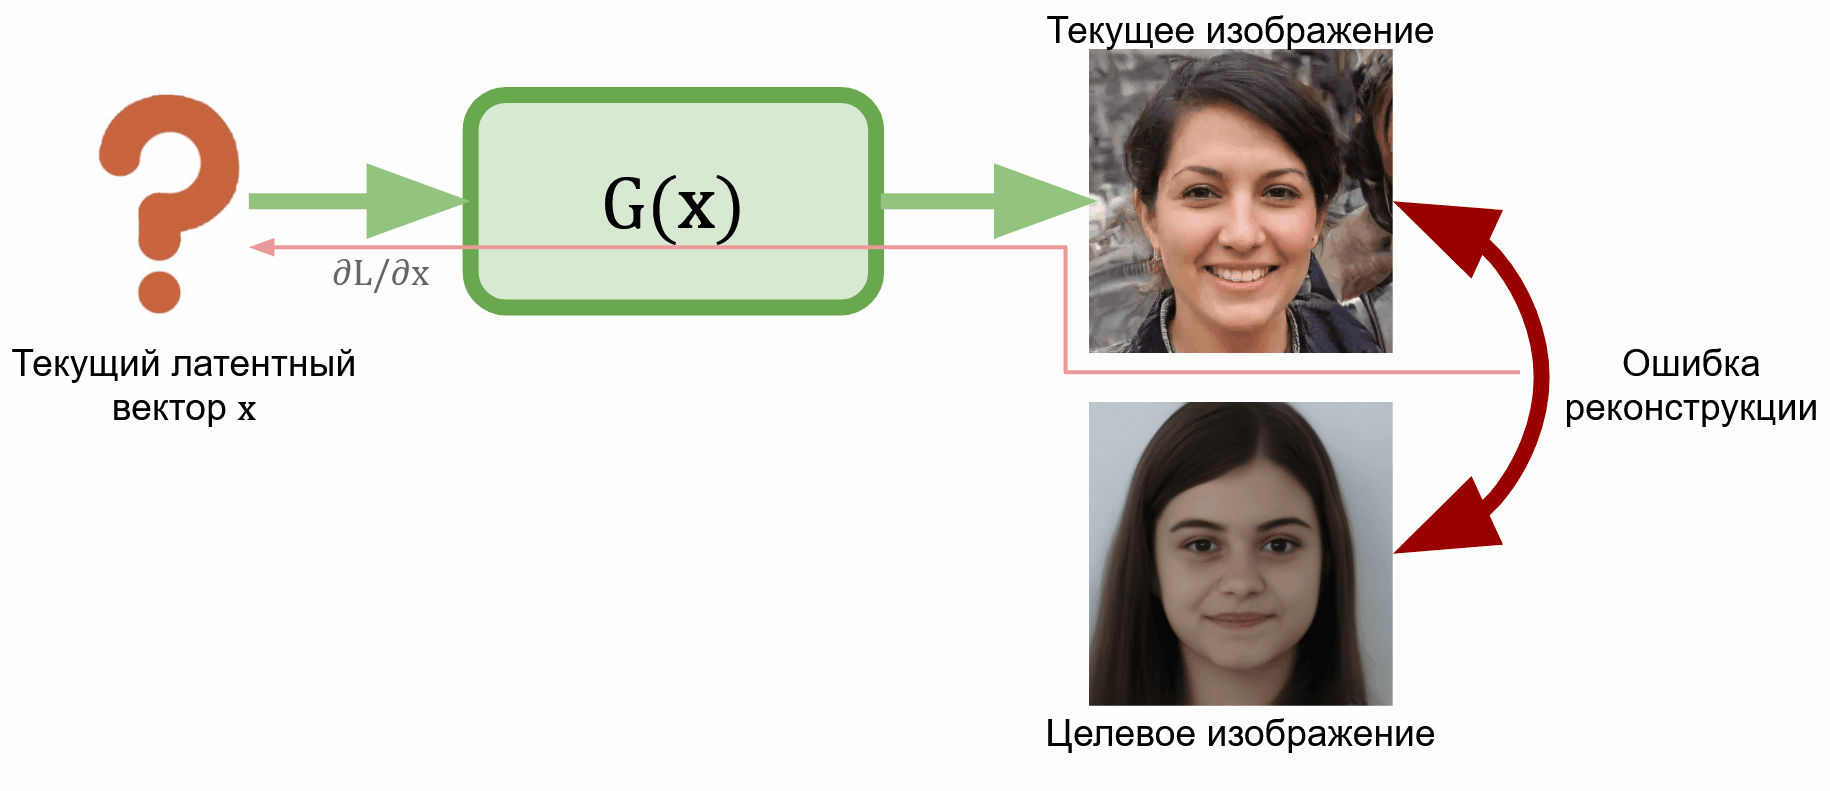
\includegraphics[width=0.9\textwidth]{optim_pipeline_ru}
    \caption{Архитектура нейронной сети для латентной оптимизации}
    \label{fig:optim_pipelin}
\end{center}
\end{figure}

В качестве функцию потерь реконструкции используется взвешенная сумма среднеквадратичной ошибки в пространстве пикселей и визуальной функции потерь (\emph{perceptual loss} \cite{Johnson2016Perceptual}).
%Здесь нужно сказать, что следуем Image2StyleGAN, что используем W+

\emph{Дальше нужно написать достаточно сложный абзац, объясняющий пространство $W+$ и оптимизацию отдельных грубых мап признаков.}
%собственно здесь описываем модификацию того, что ступенчато оптимизируемся и что это позволяет не улететь датеко от данных (см. Latent Space Oddity).


%\subsection{Алгоритм выделения семантик}
\subsection{Алгоритм выделения линейных подпространств, соответствующих семантикам изображения}
\emph{Здесь будет расписан алгоритм выделения семантик, лежащий в основе решения.}

Для выделения семантик изображения принимается предположение о линейности латентного пространства.

Рассмотрим произвольный бинарный признак, заданный дискриминативной функцией $f : \mathcal X \mapsto \{0,1\}$, определяющей наличие или отсутствие этого признака на изображении.
При справедливости этого предположения линейная интерполяция между двумя латентными векторами, соответствующими двум изображениям, на одном из которых признак присутствует, а на другом --- отсутствует, приведет к постепенному и непрерывному изменению этого признака на генерируемом изображении. 

Как показано в \cite{StyleGAN}, линейная разделимость бинарных признаков в промежуточном латентном пространстве $\mathcal{W}$ позволяет найти векторы направлений, соответствующих отдельным факторам вариации, т.е. отдельным признакам.

Для нахождения данных направлений используется следующий метод.
\begin{itemize}
    \item В качестве функции $f$ используется нейросетевой классификатор, обученный на датасете CelebA-HQ. Архитектура крассификатора аналогична архитектуре дискриминатора, используемого в \cite{progressive-growing-gan, StyleGAN}. В качестве рассматриваемых признаков были выбраны \emph{наличие улыбки} и \emph{поворот головы}.
    \item С помощью имеющегося генератора $G$ генерируется набор данных, состоящий из $20000$ изображений. Данный набор размечается с помощью классификатора $f$.
    \item На полученном наборе данных обучается линейная SVM \cite{svm} и находится оптимальная разделяющая гиперплоскость. 
\end{itemize}
Нормальный вектор полученной гиперплоскости задает направление, соответствующее рассматриваемому признаку.
%\subsection{Генерация данных}
%\subsection{Оптимальная разделяющая гиперплоскость}
%\subsection{Линейная разделимость в латентном пространстве}

\begin{figure}[h]
\begin{center}
    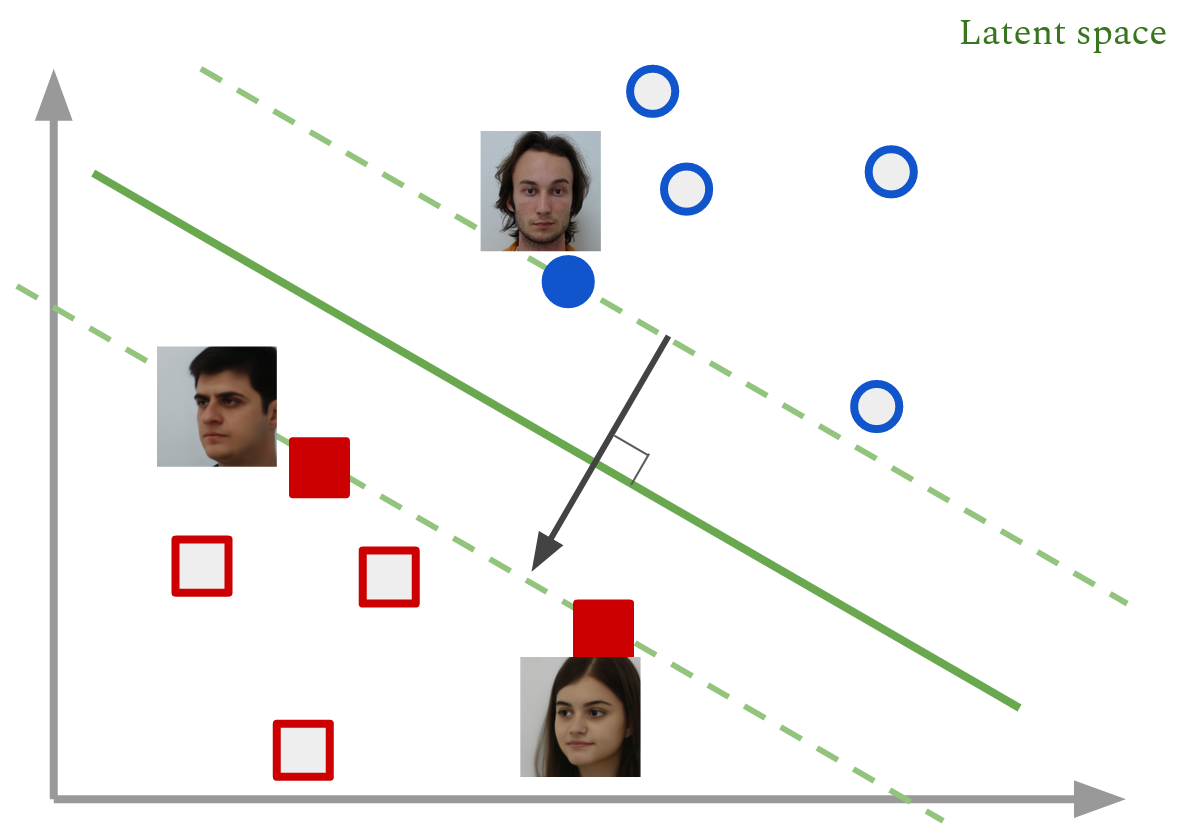
\includegraphics[width=0.7\textwidth]{boundary-SVM}
    \caption{Иллюстрация процесса нахождения векторов направлений, соответствующих отдельным факторам вариации, путем нахожения оптимальной разделяющей плоскости.}
    \label{fig:svm-boundary}
\end{center}
\end{figure}


\subsection{Алгоритм переноса лицевых признаков с изображения образца}

%Переформулировать в терминах оптимизации.

% Мы оптимизируем пока не сойдемся по одному Degree of Freedom, и при этом делаем ортогональный шаг по остальным Degree of Freedom.
На генерируемом изображении $g(\mathbf x + \alpha \mathbf n)$, полученном путем линейного сдвига в направлении полученного вектора $\mathbf n$, выбранный семантический признак будет более выражен при $\alpha > 0$, и менее выражен при $\alpha  < 0$.

%собственно здесь описываем модификацию того, что используется Face Model для введения нелинейности и сохранения личности.